\renewcommand{\theequation}{\theenumi}
\begin{enumerate}[label=\thesection.\arabic*.,ref=\thesection.\theenumi]
\numberwithin{equation}{enumi}
\item The histogram for the above data is represented in fig. \ref{fig:histogram}
\begin{figure}[!ht]
\centering
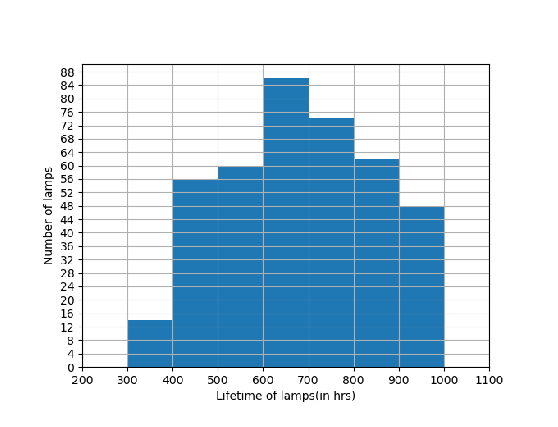
\includegraphics[width= \columnwidth]{./statistics/figs/Q41.eps}
\caption{Histogram showing No.of lamps vs. Lifetime of lamps}
\label{fig:histogram}
\end{figure}
\item From the graph, the no.of lamps having lifetime grater than 700 hrs = 74+62+48=184.
\item Download the python code for the figure from
\begin{lstlisting}
statistics/codes/Q41.py
\end{lstlisting}

\end{enumerate} 